\section{Listen}

\begin{frame}[fragile]
\frametitle{Listen}

Warum Listen?
\begin{itemize}
    \item erste Node wird \textit{head} genannt (letzte wird \textit{tail} genannt)
    \item jede Node hat einen Zeiger auf nächste Node
    \item sie sind dynamisch vergrößerbar
    \item effizient, wenn wir einfügen oder löschen wollen
\end{itemize}

\vspace{0.5cm}

\begin{center}
    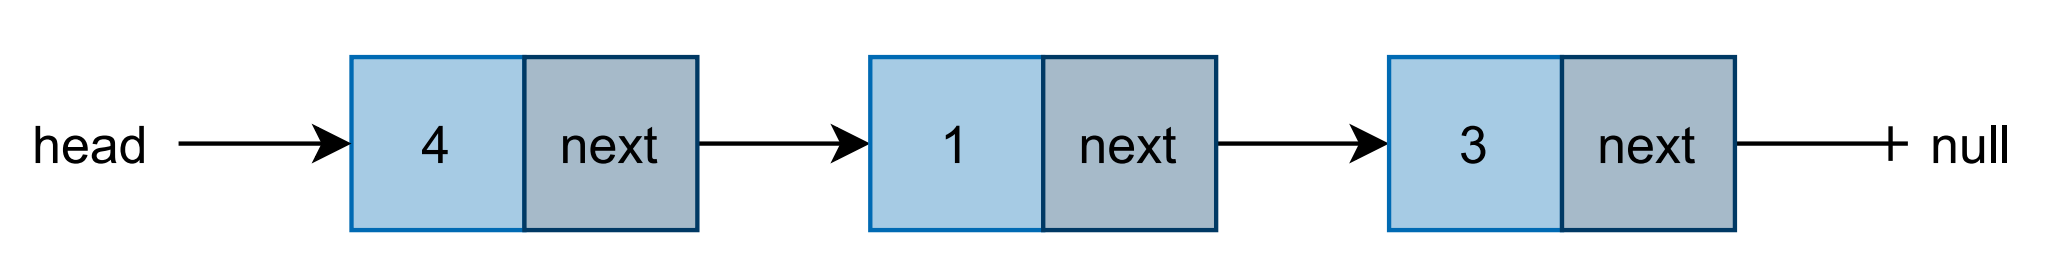
\includegraphics[width=0.9\linewidth]{images/list.png}
\end{center}
\end{frame}

\begin{frame}[fragile]
\frametitle{Listentypen}
\begin{itemize}
    \item \textbf{Einfach verkettete Liste:} Jede Node zeigt nur auf die nächste Node.
    \item \textbf{Doppelt verkettete Liste:} Jede Node zeigt auf vorherige und nächste Node.
\end{itemize}
\end{frame}


\begin{frame}[fragile]
\frametitle{Node-Klasse}
\begin{lstlisting}[language=Java]
class LinkedList {
    private Node head;

    private class Node {
        int data;
        Node next;

        Node(int data) {
            this.data = data;
            this.next = null;
        }
    }
    (...)
}
\end{lstlisting}
\end{frame}


\begin{frame}[fragile]
\frametitle{Einfügen am Anfang}
\begin{lstlisting}[language=Java]
void insertAtHead(int value) {
    Node newNode = new Node(value);
    newNode.next = head;
    head = newNode;
}
\end{lstlisting}
\end{frame}


\begin{frame}[fragile]
\frametitle{Einfügen am Ende}
\begin{lstlisting}[language=Java]
void insertAtTail(int value) {
    Node newNode = new Node(value);
    if(head == null) {
        head = newNode;
        return;
    }
    Node current = head;
    while(current.next != null) {
        current = current.next;
    }
    current.next = newNode;
}
\end{lstlisting}
\end{frame}


\begin{frame}[fragile]
\frametitle{Übersicht des Collection-Frameworks}
\begin{center}
    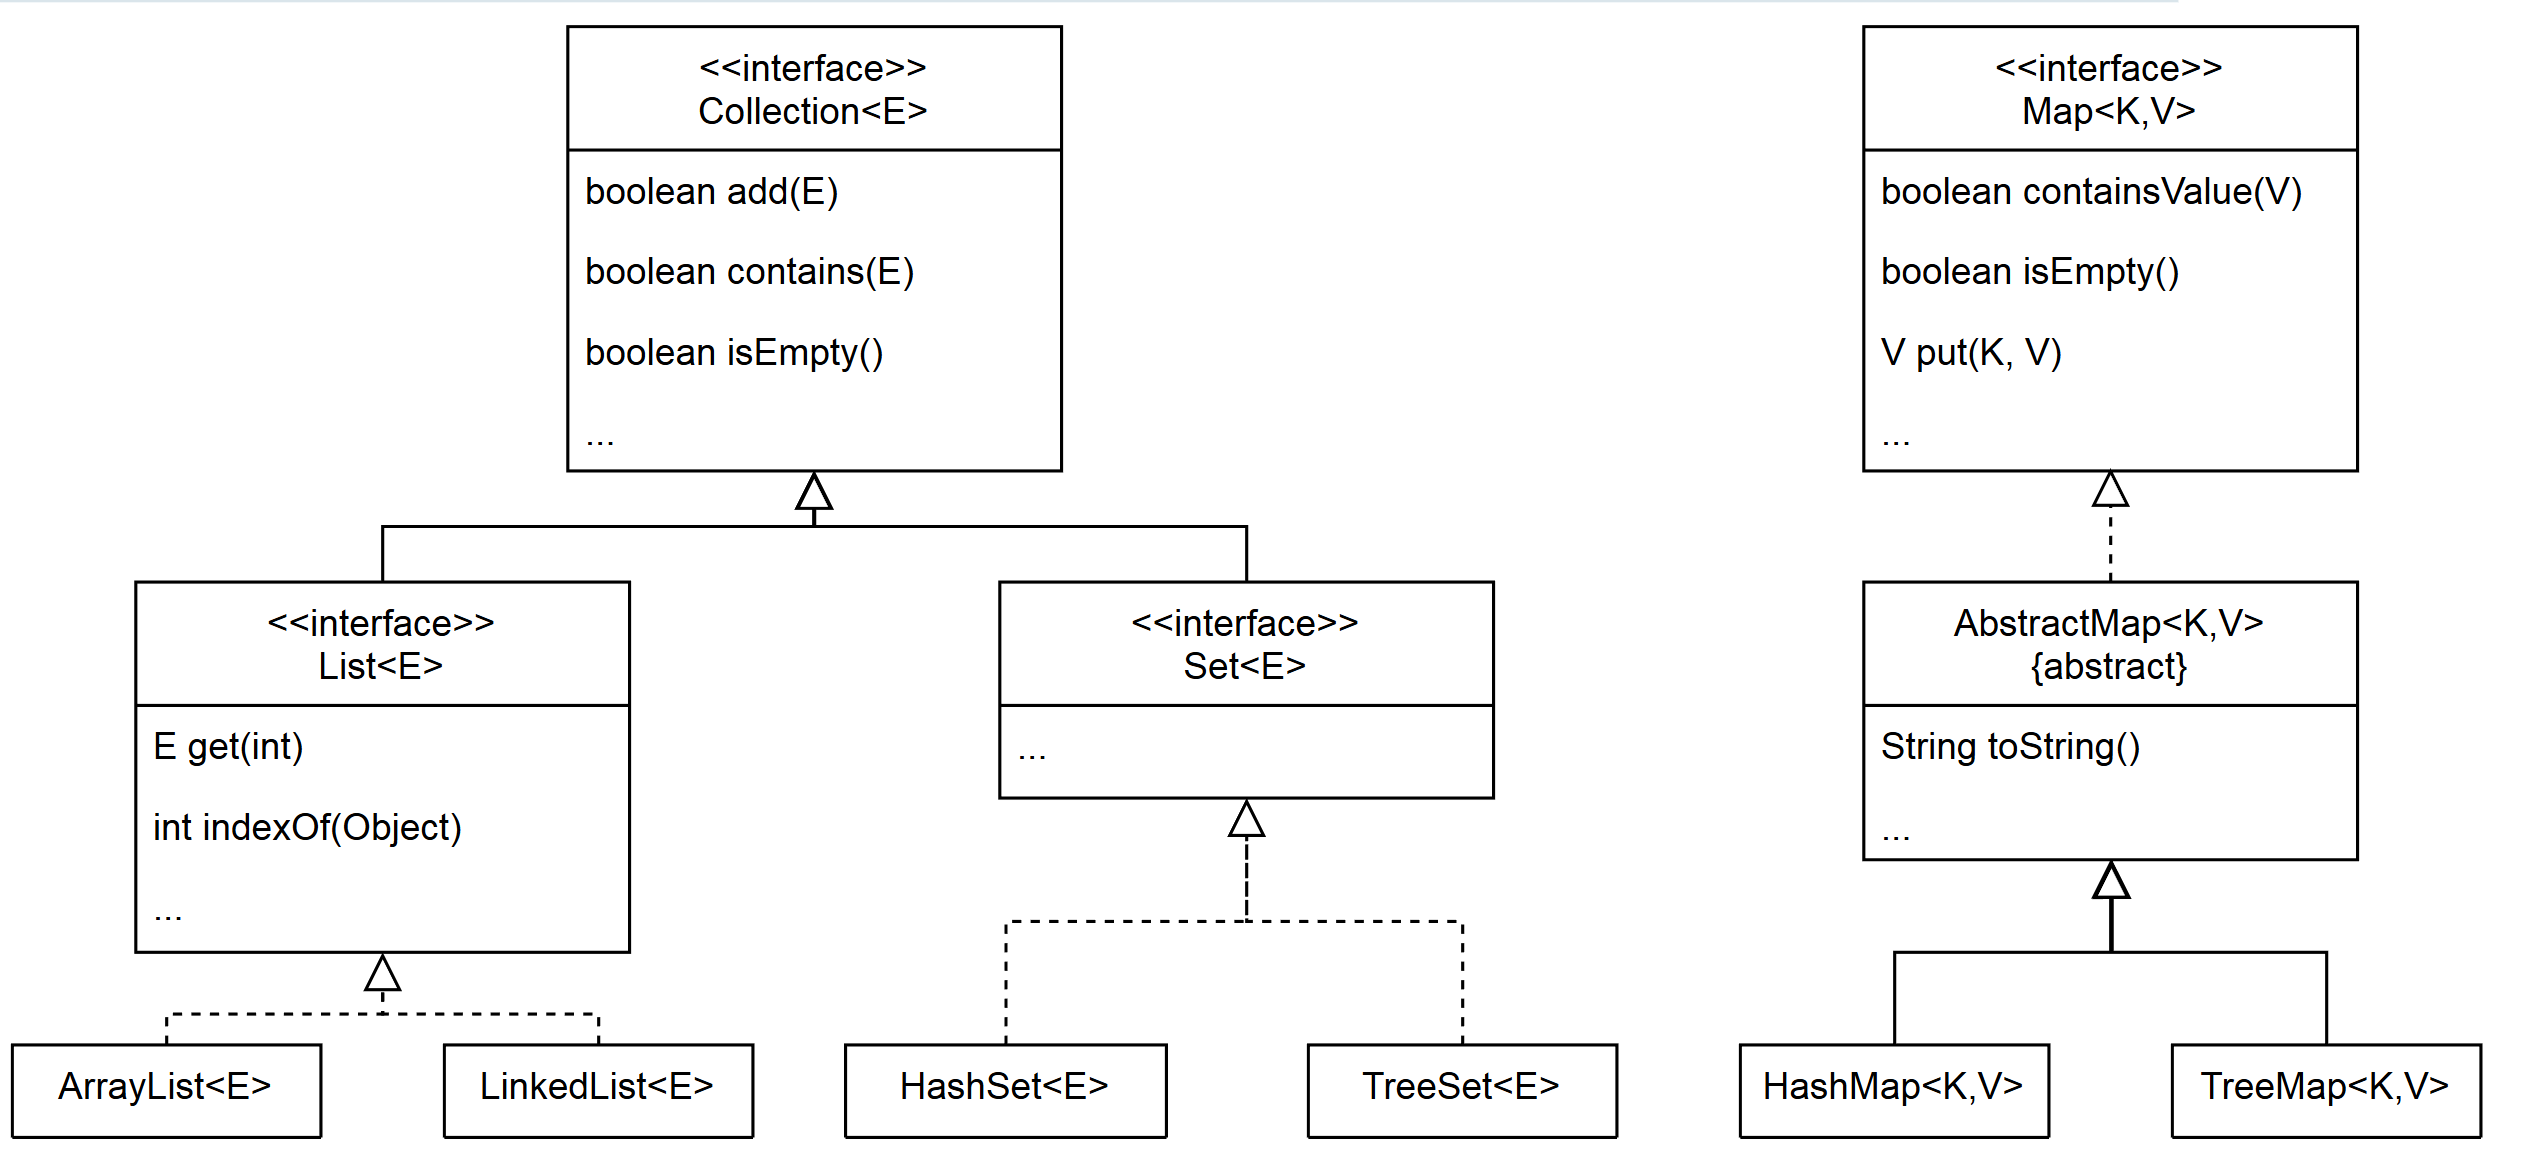
\includegraphics[width=0.9\linewidth]{images/collections.png}
\end{center}
\end{frame}






